\documentclass[12pt]{article}
\usepackage{graphicx}

\begin{document}

\section{Python Scripts Outline}

\subsection*{File Prep}

\begin{enumerate}

\item \textbf{reduce\_cube.py} \hfill \\
  Very first step. Reduce cube files from 2 GB to 64 MB cube files.

\item \textbf{time\_check\_modify.py} \hfill \\
  Used to check time differences between CODE group and INSTRUMENT group. With the modify option on it will write the time stamp in CODE to INSTRUMENT.

\item \textbf{spice\_att\_del.py} \hfill \\
  Attaches spice data to cube files. With the modify option, this script will delete cube files which do not have spice data.

\item \textbf{angle\_detect\_del.py} \hfill \\
  Detects emission angle of camera. Emission angle is the angle between ground nadir and the camera look direction. With the modify option, this script will delete cube files that are 5 degrees or greater off nadir. These images are removed for their emission angle because they represent difficulties in interest point matching and stereo correlation.

\item \textbf{rev\_print.py} \emph{(OPTIONAL)} \hfill \\
  Prints the Apollo orbit/revolution that the file belongs to. With the log option it will save all this information to file.

\item \textbf{produce\_footprints.py} \emph{(OPTIONAL)} \hfill \\
  Creates KML of footprint outlines from cubes files. Unfortunately this is slow on part of \verb#isis2gml#'s crazy upsampling. Be ready to sit an wait.

\end{enumerate}

\subsection*{Interest Point Detection}

\begin{enumerate}

\item \textbf{center\_lat\_lon\_det.py} \hfill \\
  Logs every files center LLA for next script.

\item \textbf{match\_prefilter.py} \hfill \\
  Takes in \verb#center\_lat\_lon\_det.py#'s log and then makes a list of all pairs of images that are within 10 degrees of each other on the surface. This list is used to reduce the number of pair wise matches used later on. In the future this list could be chopped up and used for distributed match processing.

\item \textbf{vwip\_generation.py} \hfill \\
  Processes cube files into tiffs (via GDAL) and then runs OBALOG on them. This script is meant only for super computer use. And should take 8 nodes about 10 minutes to process 1400 images.

\item \textbf{vwip\_filtering.py} \hfill \\
  Filter interest points so that they are not on the rims of shadows or near odd specular highlights that are custom to individual images. This is meant for super computer use only.

\item \textbf{vwip\_matching.py} \hfill \\
  Perform interest point matches. \emph{Currently broken.} This needs to use list provided by prefilter.

\end{enumerate}

\subsection*{Stereo Processing}

\begin{enumerate}

\item \textbf{stereo\_processing.py} \hfill \\
  Perform stereo processing on super computing nodes. It is expecting to use 4 stereo processes on each with 2 threads per process. Expect to spend 100 CPU hours per stereo process, so budget accordingly.

\end{enumerate}

\section*{Submitting to Pleiades}

Scripts are submitted to the super computer via the \verb#qsub# command. Notice that currently those scripts need to have their paths changed to match your system. I don't know if a build system could do this.

\section{Gathering Ground Control Points}

Ground Control Points (GCP) are 3D features used by Bundle Adjustment to fix
a solution to a previously excepted result. This is accomplished
usually by surveying input images and matching points to a global
mosaic. Currently there are 2 options provided to perform GCP creation.

\subsection*{Manually}

Gathering GCPs manually is done using part ISIS's Qnet and one part
any kind of map. The goal is to match features in the input images to
a single 3D location on a prior finished product. I usually use Google
Moon showing the Clementine Base Map.

So the work style is starting out with Qnet as usual. For every feature picked in qnet write down it's lat lon location in a file. At the end of the endeavor you should have a ISIS style cnet and lat long file that looks like so:

\begin{verbatim}
26.009808 3.603112
23.912069 2.049727
27.844959 7.315164
23.554260 6.437514
27.319273 2.905231
25.725205 5.222685
\end{verbatim}

Using gcp\_from\_net utility the above files can be turned into individual gcp files.

\begin{verbatim}
gcp_from_net ground_control.net latlon_measure.txt *.cub
\end{verbatim}

\subsection*{Automatically}

This is a shot in the dark. The idea is that given a rough estimation
of where an image was taken from; a crop from a finished mosaic can be
pulled. With this crop of the mosaic, interest point can be found
which relate specific LLA locations to pixel within the
image.

Kickbacks from this approach are that the input images which are often
high res than the mosaic must be down sampled to the mosaic
resolution. This makes life easier for the interest point algorithm as
mine don't check an infinite range in scale. Also this means GCPs are
only registered to a single image. This automatic approach will
produce a mass quantity of GCPs that only connect to single
images. It's unclear if this is good or bad.

Here's an example. This is the input image:

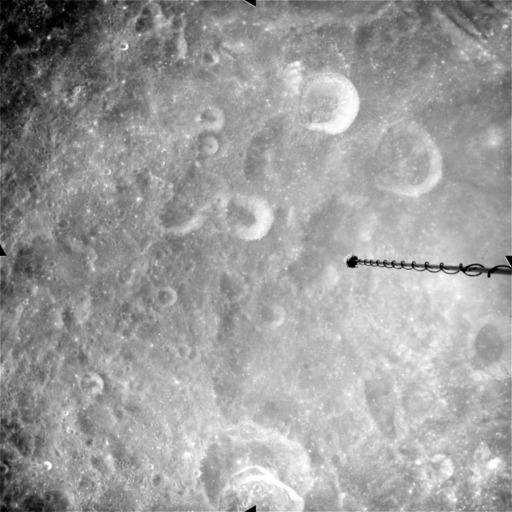
\includegraphics[width=4in]{images/AS16-M-1192.jpg}

A matching crop from the 2nd version of the Clementine 750nm mosaic is this:

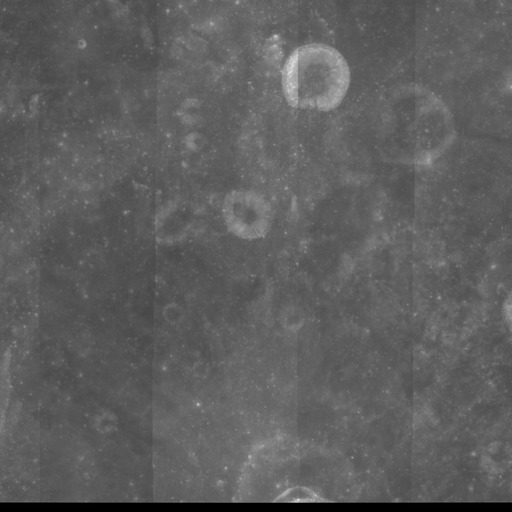
\includegraphics[width=4in]{images/AS16-M-1192_clem.jpg}

After gathering interest points, the input Apollo image can then be
warped to the Clementine. This warp is not helpful but it does prove
that the interest points made are correct.

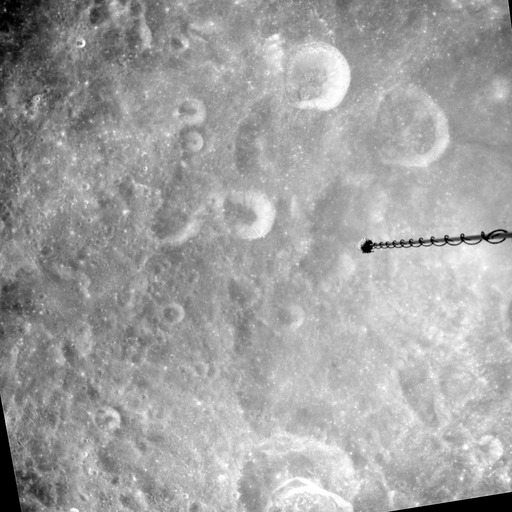
\includegraphics[width=4in]{images/aligned_AS16-M-1192.jpg}

Automatically gather GCPs are in a mass number. The utility to extract
them outputs them in a CNET format to save space. Also for the time
being the auto extraction tool only works with heavily prepared
examples.

\begin{verbatim}
echo *.cub | xargs -n 1 apollo_to_pinhole
echo *.cub | xargs -n 1 echo |
   awk -F "." '{print "from="$1".lev1.cub to="$1".lev1.tif format=TIFF"}'
   | xargs -n 3 isis2std
echo AS*.tif | xargs -n 1 mogrify -resize 1024x1024
echo *.pinhole | xargs -n 1 extract_clementine_gcp
\end{verbatim}

\end{document}
